\documentclass[16pt]{article}
\usepackage[english]{babel}
\usepackage{longtable}
\usepackage[top=1in, bottom=0.25in, left=1.25in, right=1.25in,includefoot,heightrounded]{geometry}
\usepackage{indentfirst}
\usepackage[utf8]{inputenc}
\usepackage{amsmath,amssymb}
\usepackage{graphicx,tikz}
\usepackage{hyperref}
\usepackage[colorinlistoftodos]{todonotes}
\usepackage[document]{ragged2e}
\usepackage{fancyhdr}
\usepackage{enumerate}
\usepackage{listings}
\usepackage{color}
\usepackage{flowchart}
\usepackage{hyperref}
\usetikzlibrary{arrows}

\usetikzlibrary{shapes.geometric, arrows}
\tikzstyle{startstop} = [rectangle, rounded corners, minimum width=3cm, minimum height=1cm,text centered, draw=black, fill=red!30]
\tikzstyle{decision} = [diamond, minimum width=4cm, minimum height=0.5cm, text centered, draw=black, fill=green!30]
\tikzstyle{process} = [rectangle, minimum width=3cm, minimum height=1cm, text centered, draw=black, fill=orange!30]
\tikzstyle{arrow} = [thick,->,>=stealth]
\tikzstyle{io} = [trapezium, trapezium left angle=70, trapezium right angle=110, minimum width=2cm, text width=4cm, minimum height=1cm, text centered, draw=black, fill=blue!30]

\pagestyle{fancy}
\fancyhf{}
\lhead{Myles Deslippe}
\rhead{Comp 3300 | Operating System Fundamentals}
\cfoot{\thepage}

\definecolor{MyDarkGreen}{rgb}{0.0,0.4,0.0}
\lstset{inputencoding=ansinew}
\lstset{breaklines=true} 

\begin{document}

    \section*{\centering{Operating System Structure}}

    \subsection*{The User Interface}
    \begin{itemize}
        \item \textbf{Operating systems} provide an \textbf{environment} for the \textbf{execution of programs}, and \textbf{services to those programs}.
        \item One set of \textbf{operating system services provides functions} that are helpful to the \textbf{user}.
        \item The \textbf{user interface} is the way \textbf{users interact with the operating system}.
        \item There are \textbf{two types} of \textbf{user interfaces}:
        \begin{enumerate}
            \item The \textbf{command-line interface (CLI)} is a way the \textbf{user} can \textbf{interact} with the \textbf{operating system} through a set of \textbf{commands}.
            \item The \textbf{graphical user interface (GUI)} is a way the \textbf{user} can \textbf{interact} with the \textbf{operating system} in a \textbf{graphical environment}.
        \end{enumerate}
        \item Any operating system \textbf{user interface} should allow the user to \textbf{perform file-system manipulation}, \textbf{execute programs}, and \textbf{interact with IO devices}.
        \item Additionally, the \textbf{user interface} should handle \textbf{error detection, resource allocation, and device security} behind the scenes.
        \item[] 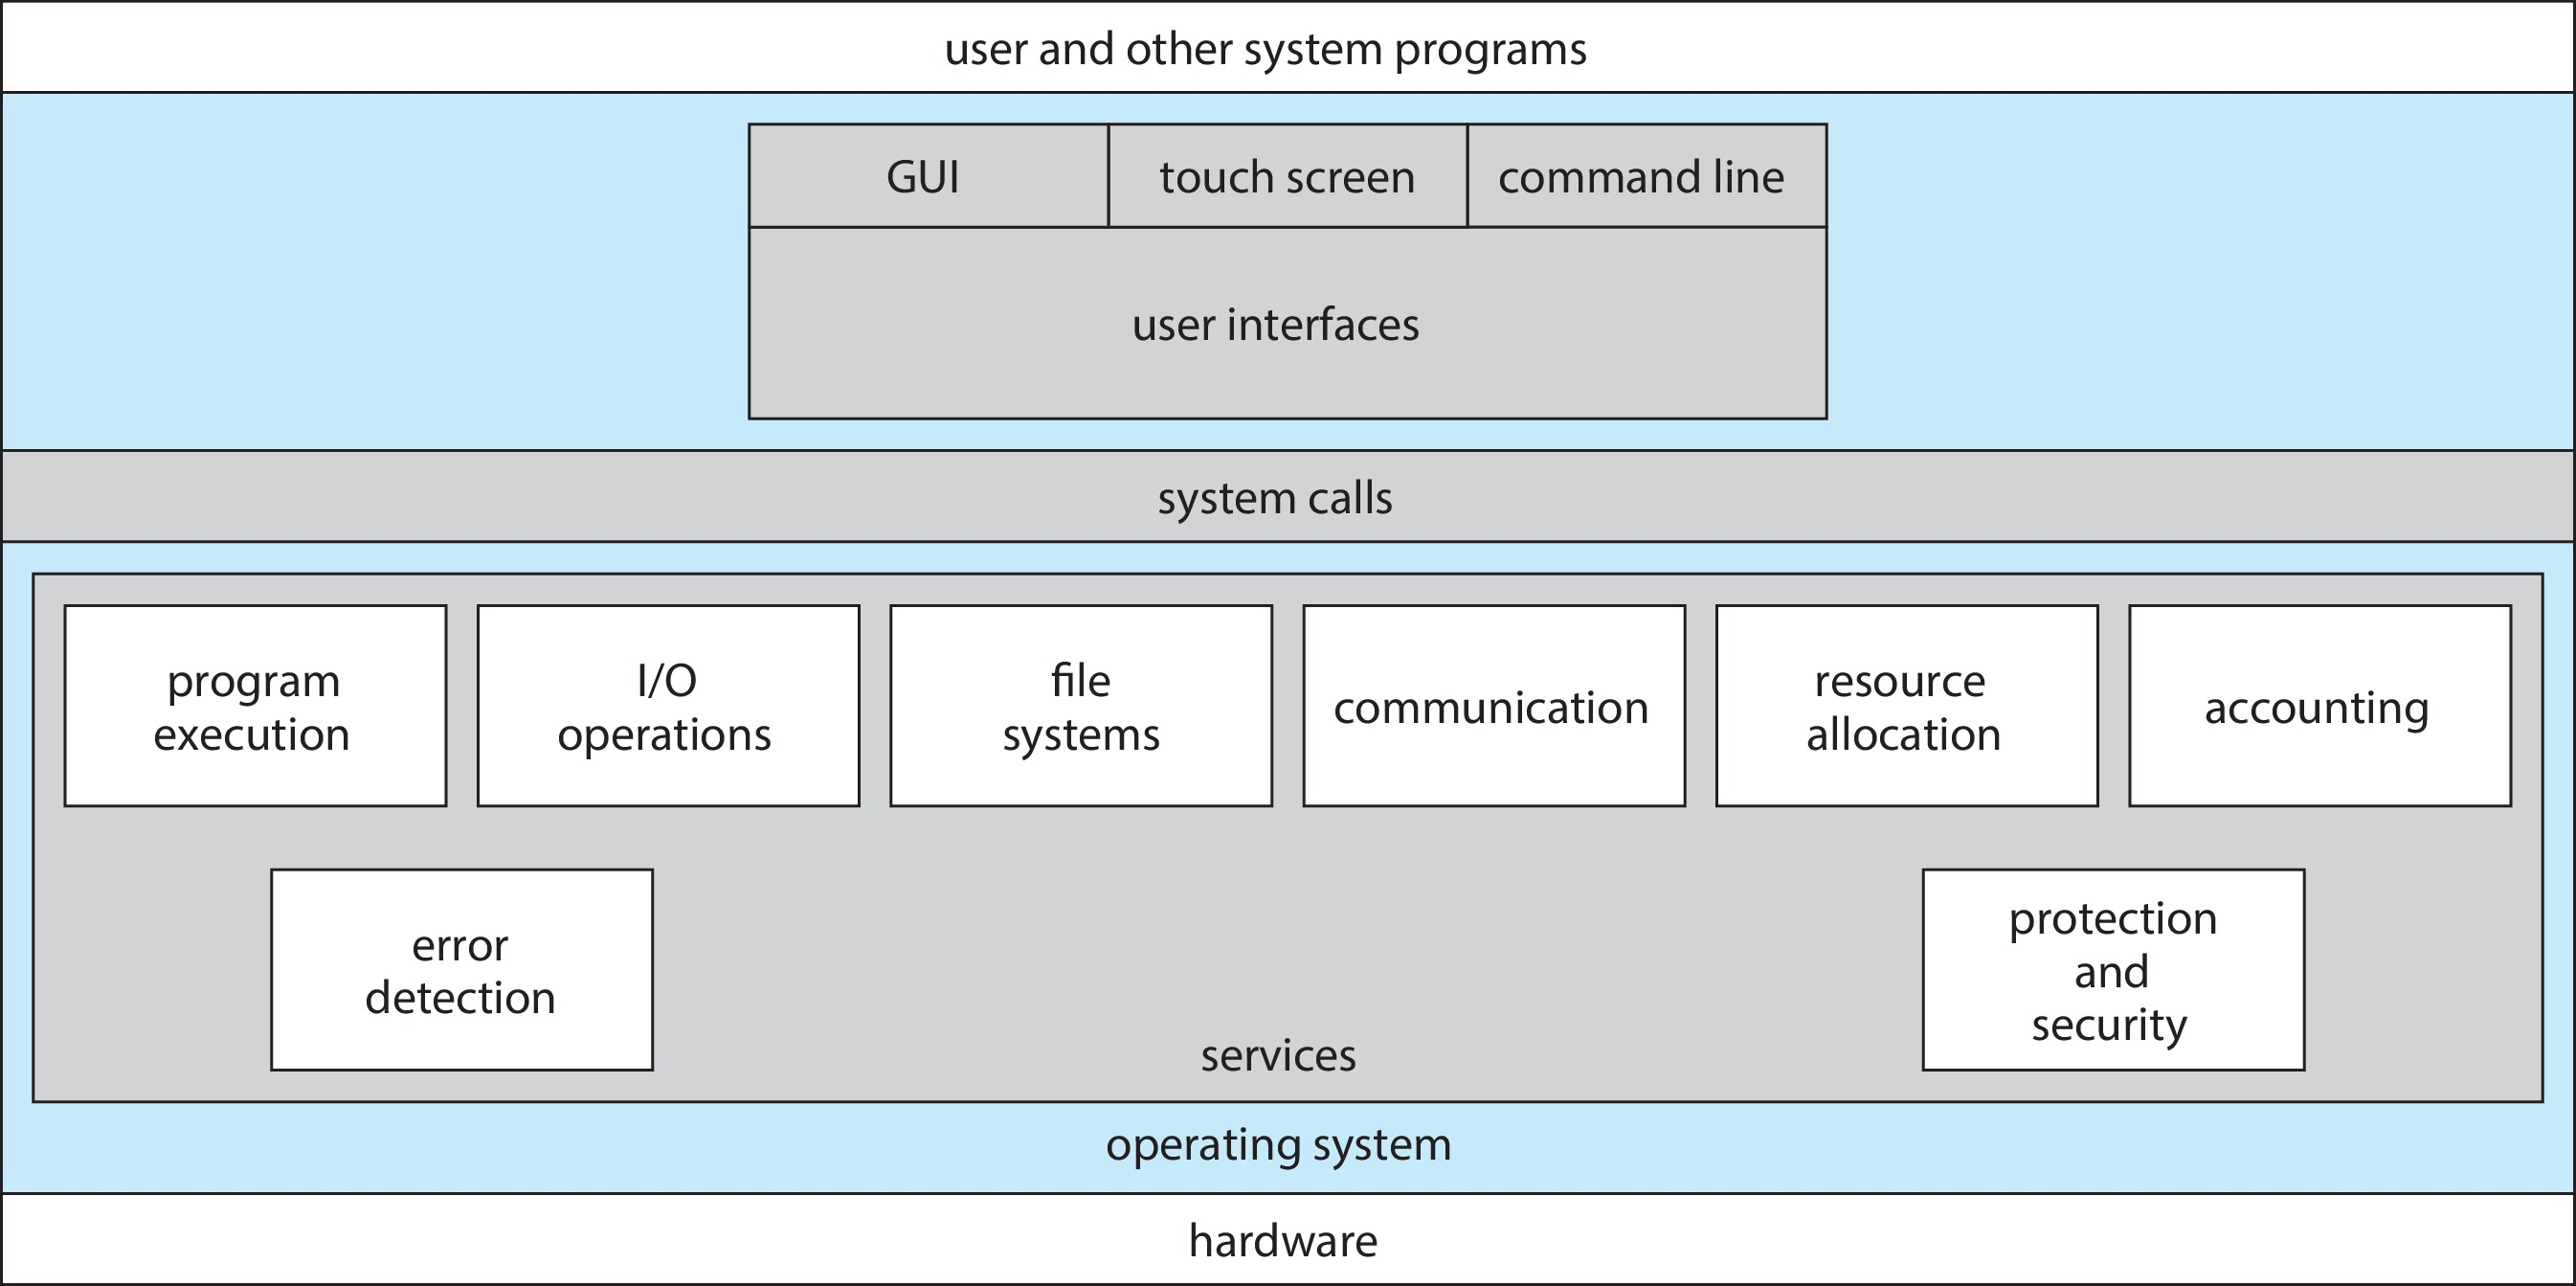
\includegraphics[height=200px]{images/User-Interface.jpg}
    \end{itemize}

\end{document}